%slide relative ad introdurre gli elementi di XML Schema Definition (XSD) 

%frame 01
\begin{frame}
	\frametitle{Elementi per la definizione degli schemi xml}
	\framesubtitle{principi XML Schema Definition}
	\addtocounter{nframe}{1}

	\begin{block}{Cos'è uno schema XML}
		Uno schema XML è un documento XML standard che descrive come deve essere realizzato un altro documento XML.
		\\ Ci riferiamo a questa tecnologia con l'acronimo XSD.
	\end{block}

	\begin{block}{A cosa serve uno Schema XML}
		I documenti XSD sono usati per validare documenti XML.
		\\ Tuttavia un documento XSD viene realizzato tramite l'uso di un vocabolario predefinito riferibile attraverso un namespace con URI standard.
	\end{block}

\end{frame}

%frame 02
\begin{frame}
	\frametitle{Elementi per la definizione degli schemi xml}
	\framesubtitle{principi XSD}
	\addtocounter{nframe}{1}

	\begin{block}{XSD Schema}
		Il termine XSD o XML Schema denota un documento XML che descrive e valida la struttura e il contenuto di un altro documento XML.
	\end{block}

	\begin{block}{XSD Schema}
		\textbf{Dichiarazione del documento (declaration) e istanza del documento (instance).}
	\end{block}

\end{frame}

%frame 03
\begin{frame}
	\frametitle{Elementi per la definizione degli schemi xml}
	\framesubtitle{principi XSD}
	\addtocounter{nframe}{1}

	\begin{block}{XSD elemento root}
		L'elemento radice di uno schema XSD è sempre l'elemento ``\texttt{<schema>}''.
		\\ Tutte le definizione devono seguire quindi l'elemento ``\texttt{<schema>}''.
	\end{block}

	\begin{block}{XSD Schema}
		Tutti gli elementi e gli attributi dello schema sono dichiarati all'interno del namespace ``\texttt{http://www.w3.org/2001/XMLSchema.}''.
		\\ Tutti i documenti XSD contengono la dichiarazione a questo namespace con prefisso convenzionale \textbf{xsd} oppoure \textbf{xs}.
	\end{block}

\end{frame}

\begin{frame}
	\frametitle{Elementi per la definizione degli schemi xml}
	\framesubtitle{principi XSD}
	\addtocounter{nframe}{1}

	\begin{block}{XSD componenti di base}
		I componenti di base di uno Schema XSD sono le dichiarazioni degli elementi e le dichiarazioni degli attributi.
	\end{block}

	\begin{block}{XSD Schema}
		\textbf{Le dichiarazioni più complesse si poggiano su queste unità: elementi e attributi.}
	\end{block}

\end{frame}

\begin{frame}
	\frametitle{Elementi per la definizione degli schemi xml}
	\framesubtitle{principi XSD}
	\addtocounter{nframe}{1}

	\begin{block}{XSD dichiarazioni}
		Scrivere un pezzo di codice XSD per descrivere e validare un elemento per un documento XML è detto \textit{element declaration}.
	\end{block}

	\begin{block}{XSD dichiarazioni di base}
		XSD permette di dichiarare elementi, attributi e di specificare il numero di figli, le occorrenze, l'ordine di apparizione, e i tipi di dati del content model.
	\end{block}

\end{frame}


\begin{frame}
	\frametitle{Elementi per la definizione degli schemi xml}
	\framesubtitle{principi XSD}
	\addtocounter{nframe}{1}

	\begin{block}{Element Types: simple and complex}
		La dichiarazione di un elemento può avere un tipo semplice (\textit{simple type}) oppure un tipo complesso (\textit{complex type}) a seconda della sua struttura e del suo contenuto.


	\end{block}

	\begin{block}{Simple Type e Complex Type}
		La dichiarazione di un elemento ha un tipo semplice se non possiede \textbf{né figli né attributi}.
		\\ La dichiarazione di un elemento ha un tipo complesso in tutti gli altri casi.
	\end{block}

\end{frame}


%frame 04
\begin{frame}
	\frametitle{Elementi per la definizione degli schemi xml}
	\framesubtitle{principi XSD}
	\addtocounter{nframe}{1}

	%\defverbatim{\xsdfirst}{%
	%\begin{tiny}
	%\begin{verbatim}
	%    <xsd:schema xmlns:xsd="http://www.w3.org/2001/XMLSchema">
	%        <xsd:element name="text"/>
	%    </xsd:schema>
	%\end{verbatim}
	%    \end{tiny}
	%   }

	%  \defverbatim{\xmlfirst}{%
	% \begin{tiny}
	%\begin{verbatim}
	%         <text>Il primo documento XML Validato</text>
	% \end{verbatim}
	% \end{tiny}
	% }


	\begin{block}{XSD esempio}
		% {\xsdfirst}
		\texttt{<xsd:schema xmlns:xsd=``http://www.w3.org/2001/XMLSchema''>}
		\\\texttt{<xsd:element name=``text''/>}
		\\\texttt{</xsd:schema>}
	\end{block}

	\begin{block}{XSD esempio elemento di tipo semplice}
		% {\xsdfirst}
		\texttt{<text>Il primo documento XML Validato</text>}
	\end{block}



\end{frame}

\begin{frame}
	\frametitle{Elementi per la definizione degli schemi xml}
	\framesubtitle{principi XSD}
	\addtocounter{nframe}{1}

	\begin{block}{XML XSD esempio}
		Il documento XML istanza dello schema XSD per essere valido deve contenere un elemento radice.
		Validare il documento XML con il relativo XSD con XMLlint.

	\end{block}

	\begin{block}{XMLlint}
		\texttt{xmllint xmlfirst.xml --schema ../schema/xsd/xsdfirst.xsd}
	\end{block}


\end{frame}

\begin{frame}
	\frametitle{Elementi per la definizione degli schemi xml}
	\framesubtitle{principi XSD}
	\addtocounter{nframe}{1}

	\begin{block}{Element Complex Types: esempio}

		%If an element contains child elements or attributes, it has a complex type.
		\texttt{
			<xsd:schema xmlns:xsd=``http://www.w3.org/2001/XMLSchema''>
			<xsd:element name=``Employee''>
			<xsd:complexType>
			<xsd:attribute name=``FirstName''/>
			</xsd:complexType>
			</xsd:element>
			</xsd:schema>
		}
	\end{block}

	\begin{block}{Element Complex Types: esempio}
		Il documento XML istanza dello schema:
		\\\texttt{<Employee FirstName="Jacob"/>}
	\end{block}

\end{frame}

\begin{frame}
	\frametitle{Elementi per la definizione degli schemi xml}
	\framesubtitle{principi XSD}
	\addtocounter{nframe}{1}

	\begin{block}{Complex Types}
		Alla base dello standard XSD ci sono le dichiarazioni degli elementi e degli attributi, ad un livello di astrazione più alto ci sono i types e i groups.

	\end{block}

	\begin{block}{Element Complex Types}
		\textbf{Un tipo complesso (Complex Type) può avere attributi e/o elementi figli.}
	\end{block}

\end{frame}

\begin{frame}
	\frametitle{Elementi per la definizione degli schemi xml}
	\framesubtitle{principi XSD}
	\addtocounter{nframe}{1}

	\begin{block}{Element Complex Types: Esempio Elemento con Figlio}
		\texttt{
			<xsd:schema xmlns:xsd=``http://www.w3.org/2001/XMLSchema''>
			<xsd:element name=``text''>
			<xsd:complexType>
			<xsd:sequence>
			<xsd:element name=``body''/>
			</xsd:sequence>
			</xsd:complexType>
			</xsd:element>
			</xsd:schema>}
	\end{block}

\end{frame}


\begin{frame}
	\frametitle{Elementi per la definizione degli schemi xml}
	\framesubtitle{principi XSD}
	\addtocounter{nframe}{1}

	\begin{block}{Espressività dell'XSD}

		\begin{itemize}
			\item Attribute Group, Element Group
			\item Order Indicators: all, sequence, choice
			\item Occurrence Indicators: minOccurs and maxOccurrs
			\item Annotation (utili per documentare le dichiarazioni)
		\end{itemize}

	\end{block}

\end{frame}

\begin{frame}
	\frametitle{Elementi per la definizione degli schemi xml}
	\framesubtitle{principi XSD}
	\addtocounter{nframe}{1}

	\begin{block}{Espressività dell'XSD}
		\begin{itemize}
			\item Data types: Built-in
			\item FACETS per una validazione oculata dei valori (elemento o un attributo).
			\item Restriction on base attribute
			\item Numeric e String Data Type
			\item Pattern facet
		\end{itemize}

	\end{block}

\end{frame}


\begin{frame}
	\frametitle{Elementi per la definizione degli schemi xml}
	\framesubtitle{principi XSD}
	\addtocounter{nframe}{1}

	\begin{block}{Element Declaration}
		Una dichiarazione di elemento (\textbf{XSD element declaration}) rappresenta un elemento nel documento XML istanza dello schema. 
		
	\end{block}

	\begin{block}{Element Declaration: Istanza XML }
		\texttt{<p>il contentuto testuale di un paragrafo</p>}
	\end{block}
	\textit{Un elemento ha un tipo semplice (\textbf{simple type}) se non ha attributi e non ha elementi figli}
\end{frame}


%% An XSD schema may contain Global and Local element declarations.

\begin{frame}
	\frametitle{Elementi per la definizione degli schemi xml}
	\framesubtitle{principi XSD}
	\addtocounter{nframe}{1}

	\begin{block}{Global and Local element declaration}
		Il vantaggio di usare dichiarazioni di elementi globali (\textbf{global element declaration})
		è che la dichiarazione può essere riferita più volte da altre dichiarazioni all'interno del documento XSD.
	\end{block}

\end{frame}


\begin{frame}
	\frametitle{Elementi per la definizione degli schemi xml}
	\framesubtitle{principi XSD}
	\addtocounter{nframe}{1}

	\begin{block}{Global element declaration: esempio}
		\texttt{<xsd:schema xmlns:xsd=``http://www.w3.org/2001/XMLSchema">
			\emph{<xsd:element name=``body''>}
			<xsd:complexType>
			<xsd:attribute name=``lang''/>
			<xsd:attribute name=``type''/>
			</xsd:complexType>
			</xsd:element>
			<xsd:element name=``text''>
			<xsd:complexType>
			<xsd:all>
			\emph{<xsd:element ref=``body''/>}
			</xsd:all>
			</xsd:complexType>
			</xsd:element>
			</xsd:schema>}
	\end{block}

\end{frame}


\begin{frame}
	\frametitle{Elementi per la definizione degli schemi xml}
	\framesubtitle{principi XSD}
	\addtocounter{nframe}{1}

	\begin{block}{Group declaration}
		Attributi e elementi possono essere raggruppati in costrutti detti \textbf{Attribute Groups} e \textbf{Element Groups}.
	\end{block}
	
	\textit{E' possibile riferirsi a questi gruppi all'interno di altre dichiarazioni ottenendo un significativo grado di riusabilità.}

\end{frame}


\begin{frame}
	\frametitle{Elementi per la definizione degli schemi xml}
	\framesubtitle{principi XSD}
	\addtocounter{nframe}{1}


	\begin{block}{Global element declaration: esempio}
		\texttt{\emph{<xsd:group name=``fileDesc''>}
			<xsd:sequence>
			<xsd:element name=``titleStmt''/>
			<xsd:element name=``publicationStmt''/>
			<xsd:element name=``sourceDesc''/>
			</xsd:sequence>
		}
	\end{block}

	\begin{block}{Global element declaration: esempio}
		\begin{center} \texttt{<xsd:group ref=``fileDesc''/>}\end{center}
	\end{block}

\end{frame}

\begin{frame}
	\frametitle{Elementi per la definizione degli schemi xml}
	\framesubtitle{principi XSD}
	\addtocounter{nframe}{1}

	\begin{block}{Element Declaration: Attributi nella dichiarazione}
		L'unico attributo \textit{obbligatorio} nella dichiarazione di elementi è l'attributo \textbf{name}.
	\end{block}

	\begin{block}{Element Declaration: Attributi - Esempio}
		\begin{center}\texttt{<xsd:element name=``TEI''/> }\end{center}
	\end{block}

\end{frame}

\begin{frame}
	\frametitle{Elementi per la definizione degli schemi xml}
	\framesubtitle{principi XSD}
	\addtocounter{nframe}{1}

	\begin{block}{Element declaration: lista Attributi}
		\begin{itemize}
			\item \textbf{name} (\textit{g-l}): il nome dell'elemento, unico attributo obbligatorio (\textit{dare nomi significativi agli elmenti})
			\item \textbf{type} (\textit{g-l}): aggiunta di un tipo di dato (\textit{data type}) (XSD ha buint-in data types)
			\item \textbf{id} (\textit{g-l}): identificatore univoco della dichiarazione dell'elemento(non ha effetti sull'istanza XML)
			\item \textbf{default} (\textit{g-l}): spcifica il valore di default di un elemento (solo se l'elemento è opzionale)
		\end{itemize}

	\end{block}

\end{frame}

\begin{frame}
	\frametitle{Elementi per la definizione degli schemi xml}
	\framesubtitle{principi XSD}
	\addtocounter{nframe}{1}

	\begin{block}{Element declaration: lista Attributi (cont.)}
		\begin{itemize}
			\item \textbf{fixed} (\textit{g-l}): valore di un elemento predefinito (``fixed'' e ``default'' sono mutuamente esclusivi)
			\item \textbf{nillable} (\textit{g-l}): indica che l'elemento è vuoto (xsd:nil nell'istanza XML del documento)
			\item \textbf{block} (\textit{g-l}): è utilizzato per controllare la sostizione degli elementi ( può assumere 4 differenti valori: \textit{substitution}, \textit{extension} \textit{restriction} e \textit{\#all})
		\end{itemize}
	\end{block}

\end{frame}

\begin{frame}
	\frametitle{Elementi per la definizione degli schemi xml}
	\framesubtitle{principi XSD}
	\addtocounter{nframe}{1}

	\begin{block}{Element declaration: lista Attributi (cont.)}

		\begin{itemize}
			\item \textbf{final} (\textit{g}): limita la dichiarazione dei gruppi di sostituzione ( può assumere 3 valori: \textit{\#all}, \textit{restriction} and \textit{extension})
			\item \textbf{abstract} (\textit{g}): un elemento astratto non può essere istanziato (è un modo per forzare la sostituzione)
			\item \textbf{substitutionGroup} (\textit{g}): è un modo per avere grande estensibilità delle dichiarazioni (facilità la creazione di nuovi tipi di elementi derivati)
			\item \textbf{minOccurs} (\textit{l}): controlla il numero di occorrenze minime degli elementi all'interno del documento XML istanza dello schema. (\textbf{minOccurs=0} indica elemento \textit{optionale}).
		\end{itemize}
	\end{block}

\end{frame}

\begin{frame}
	\frametitle{Elementi per la definizione degli schemi xml}
	\framesubtitle{principi XSD}
	\addtocounter{nframe}{1}

	\begin{block}{Element declaration: lista Attributi (cont.)}

		\begin{itemize}
			\item \textbf{maxOccurs} (\textit{l}): controlla il numero massimo di occorrenze degli elementi all'interno del documento XML istanza dello schema
			\item \textbf{ref} (\textit{l}): riferimento ad altri elementi dichiarati globalmente all'interno dello schema (riusabilità)
			\item \textbf{form} (\textit{l}): specifica se l'elemento deve essere qualificato con l'aggiunta del namespace (``qualified'' oppure ``unqualified'').
		\end{itemize}
	\end{block}

\end{frame}

\begin{frame}
	\frametitle{Elementi per la definizione degli schemi xml}
	\framesubtitle{principi XSD}
	\addtocounter{nframe}{1}

	\begin{block}{Element declaration: Attributi - Esempio }

		\texttt{
			<xsd:element name=``body''>
			<xsd:complexType>
			\emph{<xsd:sequence maxOccurs=``unbounded''>}
			\emph{<xsd:element ref=``div''/>}
			</xsd:sequence>
			</xsd:complexType>
			</xsd:element>
		}

	\end{block}


	\begin{block}{Element declaration: Attributi - Esempio }

		\texttt{
			<xsd:element name=``div'' type=``divType'' />
		}
		\texttt{
			<xsd:complexType name=``divType''>
			[...]
			</xsd:complexType>
		}

	\end{block}

\end{frame}

% fare un paio di slide spiegando a cosa serve l'attribute substitutionGroup e come si usa. (pp 114-133)

% The substitutionGroup attribute is used to declare elements capable of
%serving as variable content containers. Abstract is used to specify that the
%element cannot be instantiated directly. To instantiate such an element, a
%substitution element needs to be created. The block and final attributes are
%used to control substitution of the element. Final restricts substitution at
%schema level and block restricts it at instance level.


% Attribute Declaration
% simple example
% <xsd:schema xmlns:xsd="http://www.w3.org/2001/XMLSchema">
%   <xsd:element name="Employee">
%     <xsd:complexType>
%       <xsd:attribute name="status" />
%     </xsd:complexType>
%   </xsd:element>
% </xsd:schema>



\begin{frame}
	\frametitle{Elementi per la definizione degli schemi xml}
	\framesubtitle{principi XSD}
	\addtocounter{nframe}{1}

	\begin{block}{Attribute declaration}
		Un attributo è dichiarato utilizzando l'elemento \texttt{<xsd:attribute>}. \\ L'unico attributo obbligatorio nella dichiarazione è ``\textbf{name}''.
	\end{block}

	\begin{block}{Attribute declaration: Global vs Local}
		Quando una dichiarazione di attributo ha il livello gerarchico successivo a ``\texttt{<xsd:schema>}'' (\textit{la root dello schema}), questa dichiarazione è detta globale (\textit{global attribute declaration}. In caso contrario l'attributo è all'interno di un \textit{Complex Type}, ed è una (\textit{Local attribute declaration}).
	\end{block}

\end{frame}

\begin{frame}
	\frametitle{Elementi per la definizione degli schemi xml}
	\framesubtitle{principi XSD}
	\addtocounter{nframe}{1}
	\begin{block}{Attribute declaration}

		\texttt{
			<xsd:attribute name=``Name'' type=``xsd:string''/>
		}

	\end{block}
	\textit{Qualsiasi dichiarazione di attributo per essere effettivamente utile deve essere riportata all'interno di una dichiarazione di elemento}
\end{frame}

% tabella con gli attributi nella dichiarazione degli attributi
% "attributes of an attribute declaration"

\begin{frame}
	\frametitle{Elementi per la definizione degli schemi xml}
	\framesubtitle{principi XSD}
	\addtocounter{nframe}{1}

	\begin{block}{Attribute declaration: Attributi}
		\begin{itemize}
			\item \textbf{name} (\textit{g-l}): il nome dell'attributo, attributo obbligatorio.
			\item \textbf{id} (\textit{g-l}): l'identificativo della dichiarazione all'interno del documento XSD (non influenza l'istanza XML).
			\item \textbf{type} (\textit{g-l}): associa un tipo di dato allo spazio di valori che può assumere l'attributo.
		\end{itemize}

	\end{block}

\end{frame}


\begin{frame}
	\frametitle{Elementi per la definizione degli schemi xml}
	\framesubtitle{principi XSD}
	\addtocounter{nframe}{1}

	\begin{block}{Attribute declaration: Attributi (cont.)}
		\begin{itemize}
			\item \textbf{default} (\textit{g-l}): assegna un valore di default all'attributo (solo se l'attributo non è presente).
			\item \textbf{fixed} (\textit{g-l}): assegna un valore predefino e fisso all'attributo.
			\item \textbf{ref} (\textit{l}): riferimento ad una dichirazione di attributo globale
		\end{itemize}
	\end{block}


\end{frame}


\begin{frame}
	\frametitle{Elementi per la definizione degli schemi xml}
	\framesubtitle{principi XSD}
	\addtocounter{nframe}{1}

	\begin{block}{Attribute declaration: Attributi (cont.)}
		\begin{itemize}
			\item \textbf{use} (\textit{l}): specifica se l'attributo è opzionale o meno. Possibili valori sono \textit{optional}, \textit{required}, \textit{prohibited}
			\item \textbf{form} (\textit{l}): indica se l'attributo deve avere o meno indicato il namespace all'interno del documento XML istanza dello schema (può assumere due valori: \textit{qualified} e \textit{unqualified})
		\end{itemize}

	\end{block}

\end{frame}


\begin{frame}
	\frametitle{Elementi per la definizione degli schemi xml}
	\framesubtitle{principi XSD}
	\addtocounter{nframe}{1}

	\begin{block}{Attribute declaration: Esempio (global)}

		\texttt{
			<xsd:schema xmlns:xsd=``http://www.w3.org/2001/XMLSchema''>
			\emph{<xsd:attribute name=``analysis'' />}
			<!-- -->
			<xsd:element name=``word''>
			<xsd:complexType>
			\emph{<xsd:attribute ref=``analysis''/>}
			</xsd:complexType>
			</xsd:element>
			</xsd:schema>
		}

	\end{block}

	\textit{Global attribute declarations are useful when an attribute is declared with several validations}


\end{frame}



%% Esempio da img GlobalAttribute
%% global attribute declarations provide some sort of re-usability.

%% esempio type:
% <xsd:schema xmlns:xsd="http://www.w3.org/2001/XMLSchema">
%   <xsd:element name="Employee">
%     <xsd:complexType>
%       <xsd:attribute name="Age" type="xsd:positiveInteger"/>
%     </xsd:complexType>
%   </xsd:element>
% </xsd:schema>

%% Attribute Groups
% Attribute Groups provide a convenient means to reuse attribute declarations in multiple complex types. Attribute Groups provide a better level of reusability by grouping one or more attribute declarations into a named group. By using an attribute group, you can avoid this repetition of code. Chain of attribute group hierarchies.

\begin{frame}
	\frametitle{Elementi per la definizione degli schemi xml}
	\framesubtitle{principi XSD}
	\addtocounter{nframe}{1}

	\begin{block}{Attribute declaration: Attribute Groups}
		Definire gruppi di attributi permette di riusare le dichirazioni degli attributi in molteplici altre dichiarazioni all'interno dello schema.
		\\I gruppi di attributi permettono di avere un maggiore livello di riusabilità delle dichiarazioni.
	\end{block}

	\textit{Attraverso l'uso dei gruppi di attributi si evitano inutili ripetizioni nel codice XSD ed è possibile costruire catene di gruppi strutturate in gerarchie ben controllate}
\end{frame}


\begin{frame}
	\frametitle{Elementi per la definizione degli schemi xml}
	\framesubtitle{principi XSD}
	\addtocounter{nframe}{1}

	\begin{block}{Attribute declaration: Esercizio (global)}
		\texttt{
			%<xsd:schema xmlns:xsd=``http://www.w3.org/2001/XMLSchema''>
			<xsd:attributeGroup name=``EmpAttributes''>
			%<!-- Declaration of attribute ``name'' -->
			<xsd:attribute name=``name''>
			<xsd:simpleType>
			<xsd:restriction base=``xsd:string''>
			<xsd:maxLength value=``20''/>
			</xsd:restriction>
			</xsd:simpleType>
			</xsd:attribute>
			%<!-- Declaration of attribute ``department'' -->
			<xsd:attribute name=``department''>
			<xsd:simpleType>
			<xsd:restriction base=``xsd:string''>
			<xsd:length value=``2''/>
			</xsd:restriction>
			</xsd:simpleType>
			</xsd:attribute>
			</xsd:attributeGroup>
			%[...]
		}
	\end{block}

\end{frame}


\begin{frame}
	\frametitle{Elementi per la definizione degli schemi xml}
	\framesubtitle{principi XSD}
	\addtocounter{nframe}{1}

	\begin{block}{Attribute declaration: Esercizio (global)}
		\texttt{
			%[...]
			%<!-- Declaration of root element ``Employees'' -->
			<xsd:element name=``Employees''>
			<xsd:complexType>
			<xsd:sequence>
			%<!-- Declaration of ``Manager'' element -->
			<xsd:element name=``Manager''>
			<xsd:complexType>
			<xsd:attributeGroup ref=``EmpAttributes''/>
			</xsd:complexType>
			</xsd:element>
			%<!-- Declaration of ``department'' element -->
			<xsd:element name=``TechLead''>
			<xsd:complexType>
			<xsd:attributeGroup ref=``EmpAttributes''/>
			</xsd:complexType>
			</xsd:element>
			</xsd:sequence>
			</xsd:complexType>
			</xsd:element>
			%</xsd:schema>
		}
	\end{block}

\end{frame}

%% Data type

\begin{frame}
	\frametitle{Elementi per la definizione degli schemi xml}
	\framesubtitle{principi XSD}
	\addtocounter{nframe}{1}

	\begin{block}{XSD Data Type}
		I linguaggi di programmazione uso i tipi (\textit{data types}) per controllare i valori che può assumere una variabile e le operazioni che possono essere effettuate su quest'ultime.
	\end{block}

		\textit{In parole povere, quando si associa un data type ad una variabile si vuole restringere lo spazio di valori permesso e restringere le operazioni che possono elaborare tali valori.}
	

\end{frame}

\begin{frame}
	\frametitle{Elementi per la definizione degli schemi xml}
	\framesubtitle{principi XSD}
	\addtocounter{nframe}{1}

	\begin{block}{XSD Data Type: esempio -  dichiarazione}
		\texttt{
			<xsd:element name=``div''>
			<xsd:complexType>
			\textit{<xsd:attribute name=``type'' />}
			\emph{<xsd:attribute name=``n'' type=``xsd:integer''/>}
			</xsd:complexType>
			</xsd:element>
		}


	\end{block}

	\begin{block}{XSD Data Type: esempio - istanza}
		\texttt{<div type="chapter" n="1" />'} \textit{(corretto)}
		\\\texttt{<div type="chapter" n="uno" />'} \textit{(errato)}

	\end{block}



\end{frame}

\begin{frame}
	\frametitle{Elementi per la definizione degli schemi xml}
	\framesubtitle{principi XSD}
	\addtocounter{nframe}{1}

	\begin{block}{XSD Data Type}
		XSD supporta diversi tipi di dati, per descrivere e validare quasi tutti i valori che possono occorrere in un documento XML. 
		\\\textbf{Ma supporta anche la possibilità di derivare nuovi data types a partire da quelli disponibili (\textit{built-in}}
	\end{block}

	\begin{block}{XSD Data Type}
		I tipi di dati aiutano a descrivere un certo dato in modo più accurato, contribuendo a validarne i valori in modo più efficace.
	\end{block}
	
\end{frame}

\begin{frame}
	\frametitle{Elementi per la definizione degli schemi xml}
	\framesubtitle{principi XSD}
	\addtocounter{nframe}{1}

	\begin{block}{XSD Data Type}
		\textbf{XSD supporta una \textit{cinquantina} di tipi di dato divisi in due categorie: \textit{Primitive Data Types} e \textit{Derived Data Types}.}
	\end{block}
	
\end{frame}

\begin{frame}
	\frametitle{Elementi per la definizione degli schemi xml}
	\framesubtitle{principi XSD}
	\addtocounter{nframe}{1}

	\begin{block}{Primitive Data Types}
		Primitive Data Types sono tipi di dati dai quali sono stati derivati altri tipi di dati.
	\end{block}
	%\textit{XSD has nineteen primitive data types}


	\begin{block}{Primiteive Data Types}

		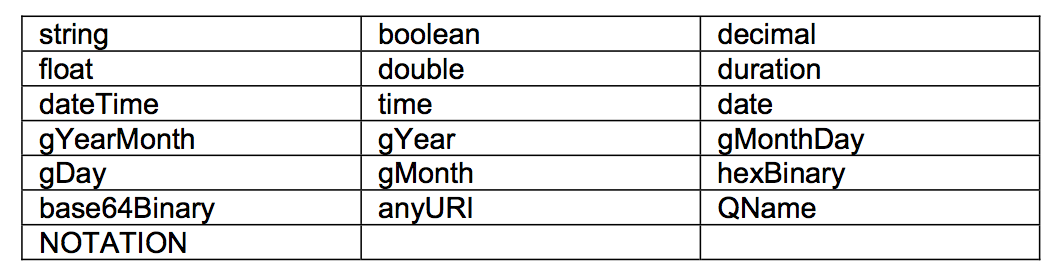
\includegraphics[width=.95\textwidth]{imgs/TabellaDataTypeXSD.png}

	\end{block}

\end{frame}

\begin{frame}
	\frametitle{Elementi per la definizione degli schemi xml}
	\framesubtitle{principi XSD}
	\addtocounter{nframe}{1}

	\begin{block}{Primitive Data Types}
		Primitive Data Types non derivano da alcun tipo di base.
	\end{block}

	\begin{block}{Derived Data Types}

		Nel sistema di tipi di XSD esistono data types che sono direttamente oppure indirettamente derivati dai Primitive Data Types.

	\end{block}

\end{frame}


\begin{frame}
	\frametitle{Elementi per la definizione degli schemi xml}
	\framesubtitle{principi XSD}
	\addtocounter{nframe}{1}

	\begin{center}
		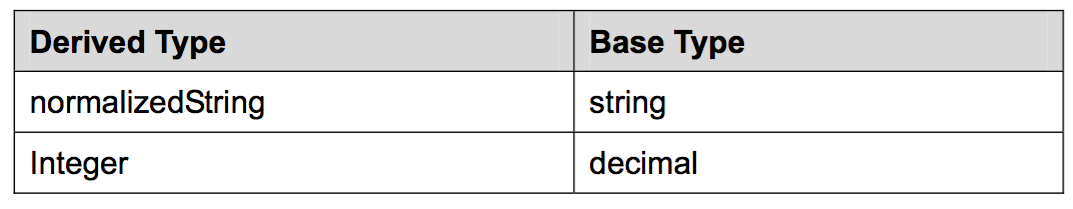
\includegraphics[width=.95\textwidth]{imgs/DerivedTypeBaseType(2types).png}
	\end{center}
	\begin{center}
		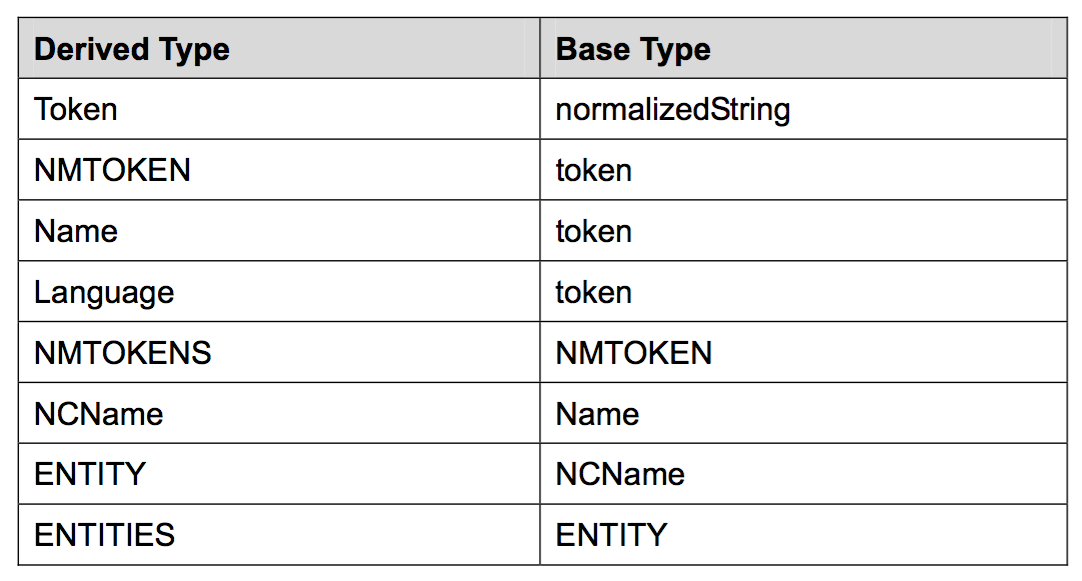
\includegraphics[width=.95\textwidth]{imgs/DerivedTypeFromDerivedType(8types).png}
	\end{center}

\end{frame}

\begin{frame}
	\frametitle{Elementi per la definizione degli schemi xml}
	\framesubtitle{principi XSD}
	\addtocounter{nframe}{1}

	\begin{center}
		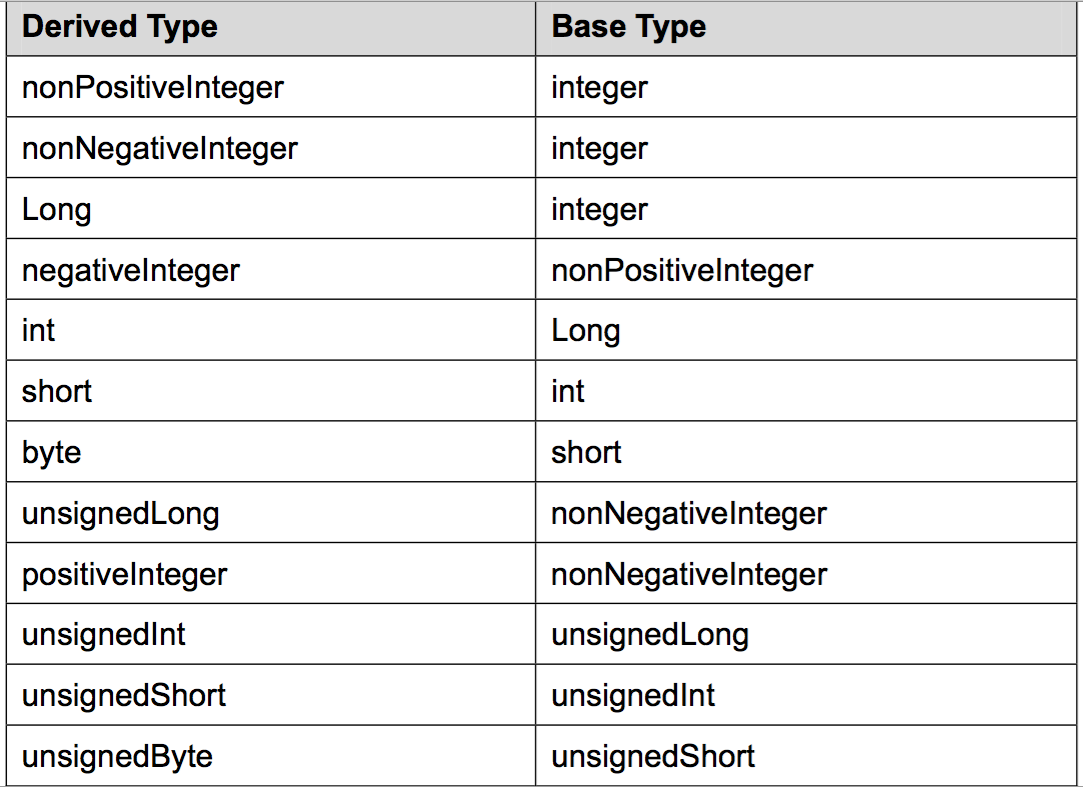
\includegraphics[width=.95\textwidth]{imgs/NumericalDerivedType(12types).png}
	\end{center}

\end{frame}



%% qualche esempio di DataType (libro XSD pagine 175 et seguenti)
% String
% Boolean
% Decimal
%% XSD decimal data type represents a subset of real numbers
% Float
%% XSD float data type is single precision 32-bit floating point type
% Double
%% XSD double data type shares the same characteristics as float except that double data type is double precision 64-bit floating point type.
% Duration
%% XSD duration data type represents duration of time
%% A duration value should always start with the letter "P" in upper case. Then each value should be separated by indicators Y (Years), M (Months), D (Days), H (Hours), M (Minutes) and S (Seconds). Letter "T" should appear as a separator between Year-Month-Day and Hour-Minute-Second.
%% esempio:
% <ElapsedTime>PT3M15S</ElapsedTime>
% DataTime
%% The format of XSD dateTime is -yyyy-mm-ddThh:mm:ss.sZ. 
% hexBinary
%% XSD hexBinary data type represents HEX encoded data.
% "This is a secret message" using the online Text-to- Hex tool available at http://tools.elitehackers.info/Hex.php.
% base64Binary
%% XSD base64Binary data type represents base64 encoded data. store binary data
%% esempio https://www.base64decode.org/
%% VGhpcyBpcyBhIHNlY3JldCBtZXNzYWdl
% QName
%% QName data type can accept a colonized value (a namespace prefix and a string value separated by a colon) only if there is a valid namespace declaration within the scope where the value is used.



\begin{frame}
	\frametitle{Elementi per la definizione degli schemi xml}
	\framesubtitle{principi XSD}
	\addtocounter{nframe}{1}

	\begin{block}{Data Type: Facets}
		Ciascun tipo di dato a una collezione di proprietà che possono essere musate per attuare validazioni aggiuntive ai valori permessi dal tipo di dato corrente.
		\\\textit{Queste proprietà sono chiamate \textbf{Facets} in XSD.}
	\end{block}

	\begin{block}{Data Type: Facets}
		Ogni tipo ha un insieme stabilito di Facets che controllano una certa proprietà o una certa caratteristica del tipo di dato considerato.
	\end{block}

\end{frame}

\begin{frame}
	\frametitle{Elementi per la definizione degli schemi xml}
	\framesubtitle{principi XSD}
	\addtocounter{nframe}{1}

	\begin{block}{Data Type: Facets Esempio}
		\texttt{
			%<xsd:schema xmlns:xsd=``http://www.w3.org/2001/XMLSchema''>
			<xsd:element name=``name''>
			<xsd:complexType>
			<xsd:attribute name=``type''>
			<xsd:simpleType>
			\emph{<xsd:restriction base=``xsd:string''>}
			\emph{<xsd:length value=``15''/>}
			</xsd:restriction>
			</xsd:simpleType>
			</xsd:attribute>
			</xsd:complexType>
			</xsd:element>
			%</xsd:schema>
		}

	\end{block}

\end{frame}

\begin{frame}
	\frametitle{Elementi per la definizione degli schemi xml}
	\framesubtitle{principi XSD}
	\addtocounter{nframe}{1}

	\begin{block}{Data Type: Facets Esempio}
		\texttt{
		%<xsd:schema xmlns:xsd=``http://www.w3.org/2001/XMLSchema''>
		<xsd:element name=``name''>
		<xsd:complexType>
		<xsd:attribute name=``type''>
		<xsd:simpleType>
		\emph{<xsd:restriction base=``xsd:string''>}
		\emph{<xsd:patter value=``[A-Za-z]+''/>}
		</xsd:restriction>
		</xsd:simpleType>
		</xsd:attribute>
		</xsd:complexType>
		</xsd:element>
		%</xsd:schema>
		}

	\end{block}

\end{frame}

\begin{frame}
	\frametitle{Elementi per la definizione degli schemi xml}
	\framesubtitle{principi XSD}
	\addtocounter{nframe}{1}

	\begin{center}
		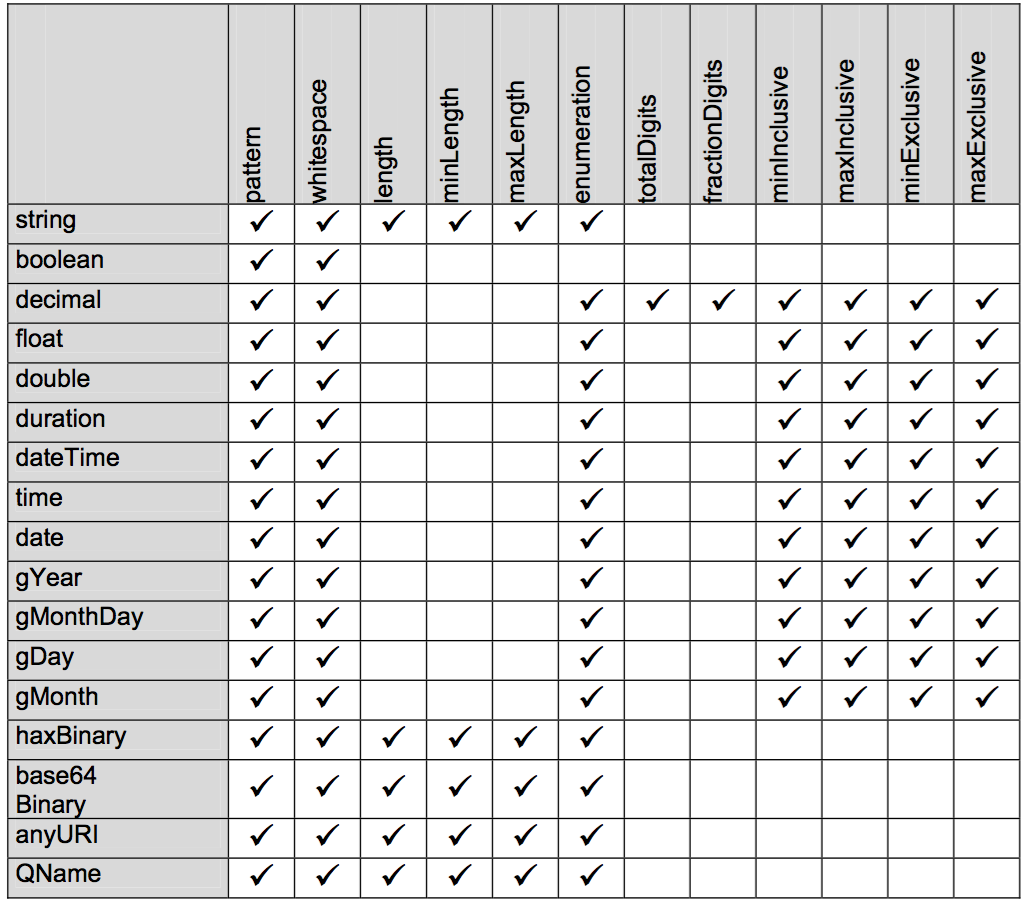
\includegraphics[width=.8\textwidth]{imgs/SchemaDataTypeFacets.png}
	\end{center}

\end{frame}



%Simple Type vs Complex Type

\begin{frame}
	\frametitle{Elementi per la definizione degli schemi xml}
	\framesubtitle{principi XSD}
	\addtocounter{nframe}{1}

	\begin{block}{Simple Type vs Complex Type}

		La differenza sostanziale tra un tipo semplice (\textit{simple types}) e un tipo complesso (\textit{complex types}) è che solo un tipo complesso può avere elementi figli e attributi.

	\end{block}

	\begin{block}{Simple Type vs Complex Type}

		Le entità \textit{simple type} possono trattare solo valori destrutturati. 
		\\Sia gli elementi sia gli attributi possono essere simple type.

	\end{block}

\end{frame}


% Simple types can only store a value. An element or attribute can have a simple type.
% Simple Types can be declared globally or locally. When a simple type is declared globally, it must always have a name.
% When a Simple Type is declared within the scope of an element or attribute it is a local declaration.
%% esempio (simpleTypeGlobalLocal)

\begin{frame}
	\frametitle{Elementi per la definizione degli schemi xml}
	\framesubtitle{principi XSD}
	\addtocounter{nframe}{1}

	\begin{center}
		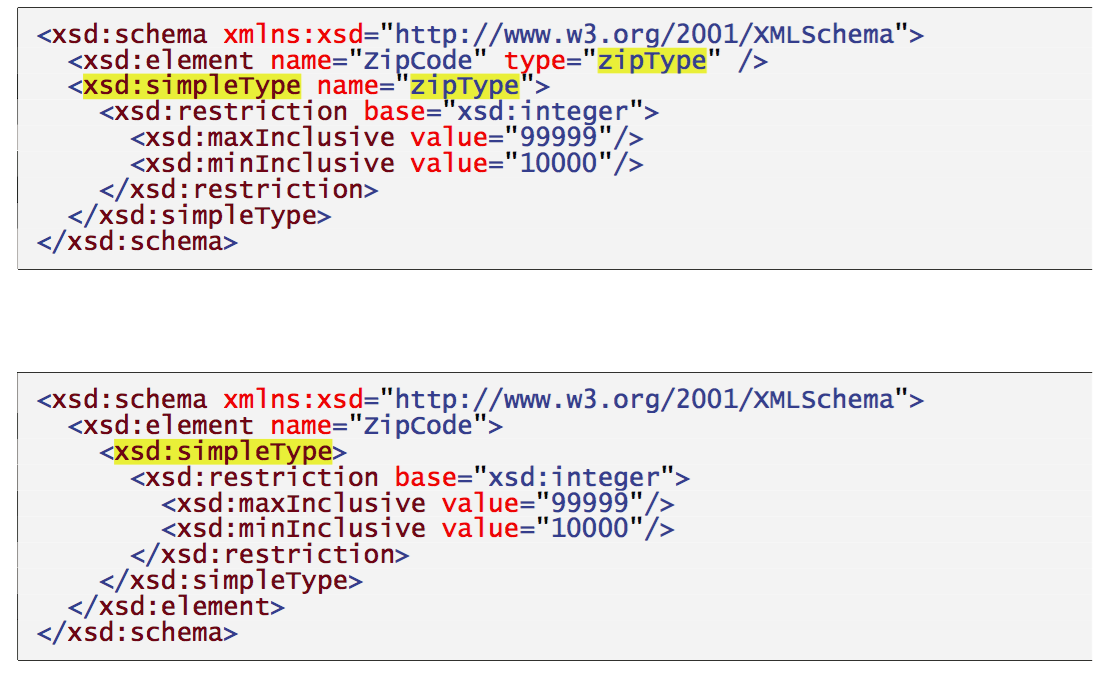
\includegraphics[width=.95\textwidth]{imgs/SimpleTypeGlobalLocal.png}
	\end{center}
	\textit{Simple Types can be declared \textbf{globally} or \textbf{locally}}

\end{frame}


\begin{frame}
	\frametitle{Elementi per la definizione degli schemi xml}
	\framesubtitle{principi XSD}
	\addtocounter{nframe}{1}

	\begin{block}{Global simple types}
		le definizioni di tipi globali sono utili per il riuso del codice e per mantenere ed organizzare al meglio una schema XSD ampio.
	\end{block}

	\textit{Molto utili quando bisogna uniformare un insieme di validazioni e manutenerle in modo coerente}

\end{frame}


\begin{frame}
	\frametitle{Elementi per la definizione degli schemi xml}
	\framesubtitle{principi XSD}
	\addtocounter{nframe}{1}

	\begin{block}{simple types: esercizio}
		\texttt{
			<xsd:simpleType name=``chapterNumberType''>
			<xsd:restriction base=``xsd:integer''>
			<xsd:maxInclusive value=``1000''/>
			<xsd:minInclusive value=``1''/>
			</xsd:restriction>
			</xsd:simpleType>
		}
	\end{block}

	\begin{block}{simple types: esercizio}
		\texttt{
			<xsd:element name=``item''>
			<xsd:complexType>
			<xsd:attribute name=``originalChapter'' type=``chapterNumberType''/>
			</xsd:complexType>
			</xsd:element>
		}
	\end{block}
\end{frame}


% Deriving

\begin{frame}
	\frametitle{Elementi per la definizione degli schemi xml}
	\framesubtitle{principi XSD}
	\addtocounter{nframe}{1}

	\begin{block}{simple types: deriving}
		Un nuovo tipo può essere derivato da un tipo già dichiarato (primitivo o meno) ed ereditarne le caratteristiche.
	\end{block}

	\begin{block}{simple types example}
		\begin{itemize}
			\item Derive by restriction
			\item Derive by list
			\item Derive by Union
		\end{itemize}
	\end{block}

\end{frame}

\begin{frame}
	\frametitle{Elementi per la definizione degli schemi xml}
	\framesubtitle{principi XSD}
	\addtocounter{nframe}{1}

	\begin{block}{simple types: deriving}
		Identificare il \textbf{tipo di dato di base} e aggiungere le dichiarazioni di \textbf{restrizione} e le \textbf{regole di validazione} che si reputano utili.
	\end{block}

\end{frame}

\begin{frame}
	\frametitle{Elementi per la definizione degli schemi xml}
	\framesubtitle{principi XSD}
	\addtocounter{nframe}{1}

	\begin{block}{simple types: deriving by Restriction}
		A restriction is defined by adding
		Un restrizione si definisce aggiungendo \textbf{``xsd:restriction''} alla dichiarazione del \textit{Simple Type}. 
	\end{block}

	\textbf{Ciascun tipo di dato possiede una collezione di proprietà (facets) attraverso le quali definire la restrizione voluta.}

\end{frame}

\begin{frame}
	\frametitle{Elementi per la definizione degli schemi xml}
	\framesubtitle{principi XSD}
	\addtocounter{nframe}{1}

	\begin{block}{simple types: deriving by Restriction}
		\texttt{
			<xsd:simpleType name=``signatureType''>
			\emph{<xsd:restriction base=``xsd:integer''>}
			\emph{<xsd:totalDigits value=``5''/>}
			</xsd:restriction>
			</xsd:simpleType>
		}
	\end{block}

	\begin{block}{simple types: deriving by Restriction}
		\texttt{
			<xsd:element name=``signature'' type=``signatureType''>
		}
		
		
		\texttt{
			<signature>12345</sgnature>
		} \textit{(valido)}
		\\\texttt{
			<signature>123ab</signature>
		} \textit{(non valido)}
	\end{block}
\end{frame}

% Another way of creating a new Simple Type is by deriving by List: 

\begin{frame}
	\frametitle{Elementi per la definizione degli schemi xml}
	\framesubtitle{principi XSD}
	\addtocounter{nframe}{1}

	\begin{block}{simple types: deriving by List}
		Un data type può contenere una lista di valori separata da spazi
	\end{block}

	\begin{block}{simple types: deriving by List}
		\texttt{<xsd:simpleType name=``chapterNumberList''>
			\emph{<xsd:list itemType=``xsd:integer'' />}
			</xsd:simpleType>}
		\\\texttt{
			<xsd:element name=``chapters'' type=``chapterNumberList'' />}
		\\\texttt{
			\textit{<chapters>1 53 60 61 205 409</chapters>}}
	\end{block}

\end{frame}

\begin{frame}
	\frametitle{Elementi per la definizione degli schemi xml}
	\framesubtitle{principi XSD}
	\addtocounter{nframe}{1}

	\begin{block}{simple types: deriving by Union}
		Un tipo derivato può accettare valori di qualsiasi tipo dichiarato nella derivazione.
	\end{block}

	\begin{block}{simple types: deriving by Union}
		\texttt{<xsd:simpleType name=``ZipCityUnion''>
			<xsd:union>
			<xsd:simpleType>
			<xsd:restriction base="ZipType"/>
			</xsd:simpleType>
			<xsd:simpleType>
			<xsd:restriction base="CityType"/>
			</xsd:simpleType>
			</xsd:union>
			</xsd:simpleType>}

	\end{block}

\end{frame}



% A third method of deriving a simple type is by union. The derived type can store the values acceptable to any of the base types from which the new type is derived.
% esempio:

% <xsd:simpleType name="ZipCityUnion">
%  <xsd:union>
%    <xsd:simpleType>
%      <xsd:restriction base="ZipType"/>
%    </xsd:simpleType>
%    <xsd:simpleType>
%      <xsd:restriction base="CityType"/>
%    </xsd:simpleType>
%  </xsd:union>
% </xsd:simpleType>

% The value will be accepted only if it validates successfully with one of the base types.

% It is not allowed to make the value space of a derived type less restrictive than the base type.

\begin{frame}
	\frametitle{Elementi per la definizione degli schemi xml}
	\framesubtitle{principi XSD}
	\addtocounter{nframe}{1}

	\begin{block}{simple types: deriving}
		I valori sono accettati solo se sono validi per uno dei tipi dichiarati nella derivazione.
	\end{block}

	\begin{block}{simple types: deriving}
		Nei costrutti di derivazione\textit{ non è permesso aumentare lo spazio dei valori consentiti}.
		\\\textbf{Non è possibile} quindi definire regole meno restrittive di quelle che caratterizzano il tipo di base.
	\end{block}
\end{frame}


% each XSD data type has a certain number of facets that control its value space.
% When we derive a new Simple Type from another, the new type will inherit all the facets of the base type. You can set the "fixed" attribute of the given facets to "true" to make sure that the derived types do not modify those facets.

\begin{frame}
	\frametitle{Elementi per la definizione degli schemi xml}
	\framesubtitle{principi XSD}
	\addtocounter{nframe}{1}

	\begin{block}{simple types: deriving facets}
		\textbf{Quando si deriva un tipo semplice da un altro tipo semplice, tutte le facets vengono ereditate.}
	\end{block}

	\begin{block}{simple types: deriving facets}
		
		E' possibile utilizzare l'attributo \textbf{fixed} di una data proprietà (facets) a \textbf{true} per assicurare che la proprietà stessa non venga modificata dal tipo derivato.
	\end{block}

\end{frame}


\begin{frame}
	\frametitle{Elementi per la definizione degli schemi xml}
	\framesubtitle{principi XSD}
	\addtocounter{nframe}{1}

	\begin{block}{Simple types: controllare la derivazione}
		XSD ha anche un meccanismo per controllare e proteggere (vietare) un tipo dall'essere derivato.
		\\ Si impiega l'attributo \textbf{final} della dichiarazione di simple type.
	\end{block}

\end{frame}

\begin{frame}
	\frametitle{Elementi per la definizione degli schemi xml}
	\framesubtitle{principi XSD}
	\addtocounter{nframe}{1}

	\begin{block}{controllare la derivazione: l'attributo final}
		\begin{itemize}
			\item restriction
			\item list
			\item union
			\item extension
			\item \#all
		\end{itemize}
	\end{block}

\end{frame}


\begin{frame}
	\frametitle{Elementi per la definizione degli schemi xml}
	\framesubtitle{principi XSD}
	\addtocounter{nframe}{1}

	\begin{block}{Simple types: controllare la derivazione - esempio}
		\texttt{
			<xsd:schema xmlns:xsd=``http://www.w3.org/2001/XMLSchema''>
			\emph{<xsd:simpleType name=``zipType'' final=``restriction union list extension''>}
			<xsd:restriction base=``xsd:integer''>
			\emph{<xsd:maxInclusive value=``99999'' fixed=``true''/>}
			<xsd:minInclusive value=``10000''/>
			</xsd:restriction>
			</xsd:simpleType>
			</xsd:schema>
		}
	\end{block}

\end{frame}

\begin{frame}
	\frametitle{Elementi per la definizione degli schemi xml}
	\framesubtitle{principi XSD}
	\addtocounter{nframe}{1}

	\begin{block}{Simple types: controllare la derivazione - esempio}
		Il termine estensione si riferisce alla possibilità di derivare un nuovo tipo che risulta essere complex type da un tipo base simple type.
	\end{block}

	\begin{block}{Simple types: controllare la derivazione - esempio}
		Quando l'attributo  \textbf{final} ha valore \textbf{\#all}, il Simple Type non puà essere derivato in alcun modo.
	\end{block}

\end{frame}


% Defining Enumerations
% Sometimes we will come across requirements where we need to apply a certain restriction to an element or attribute so that only a set of predefined values can be stored. 

% XSD Built-in Data Types: Primitive and Derived Data Types
% Facets of built-in data types
% XSD Built-in Derived data types
%% XSD has twenty-five such data types that derive directly or indirectly from one of the Primitive Data types
% xsd:integer is derived from xsd:decimal by restriction
% esempio

%<xs:simpleType name="integer" id="integer">
%  <xs:annotation>
%     <xs:documentation
%       source="http://www.w3.org/TR/xmlschema-2/#integer"/>
%   </xs:annotation>
%   <xs:restriction base="xs:decimal">
%     <xs:fractionDigits fixed="true" value="0"
%                        id="integer.fractionDigits"/>
%     <xs:pattern value="[\-+]?[0-9]+"/>
%   </xs:restriction>
%  </xs:simpleType>

% fractionDigits is a facet exposed by all numeric data types and it restricts the number of decimal places in the value. 
% The attribute fixed indicates that any type that derives from integer is not allowed to modify the value of fractionDigits facet.
% It applies a pattern restriction to validate the format of the value.
% as with integer, each of the XSD built-in derived data types derives from one of the Primitive Types directly or indirectly.

% Facets of Data Types
%% Each data type has a certain set of characteristics that can be used to perform additional validations on the value. Each of the XSD data types has a certain number of such properties that add additional restrictions on the value. These properties are called facets in XSD. Not all data types support the same facets.

% list of all the facets supported by the different data types of XSD.
% length restricts the number of characters a value can accept.
% minLength defines the minimum length of the value
% maxLength defines the maximum length of the value
% pattern specifies a Regular Expression to validate the value.
% enumeration is used to restrict the values to a set of predefined choices
% whitespace defines the way whitespaces is processed by the schema processor (Preserve, replace, collapse).
% totalDigits restricts the number of digits the type can hold (cifre intere + decimali)
% fractionDigits restricts the number of digits in the decimal part of the value
% maxInclusive specifies the highest value the type can accept
% minInclusive specifies the highest numeric value the type can accept, excluding the value specified in the restriction.
% maxExclusive defines the lowest value that the type can accept.
% minExclusive defines the minimum value that the type can accept, excluding the value specified in the restriction

%% foto della tabella (schemaDatatypeFacets)

%% Tipi di dati xsd derivati da tipi di dati primitivi (25 in totale)
%% immagini per i tipi e esempi di catena di derivazione (DerivedTypeBaseType, DerivedTypeFromDerivedType, NumericalDerivedType, NumericalGrafico, String-Grafico).

% complex type
\begin{frame}
	\frametitle{Elementi per la definizione degli schemi xml}
	\framesubtitle{principi XSD}
	\addtocounter{nframe}{1}

	\begin{block}{Complex Type}
		Un tipo coomplesso (\textbf{complex type}) può essere strutturato e quindi avere figli e avere attributi.
		% an element has a Simple Type, it cannot have child elements or attributes. It can store only a text value.

	\end{block}

	\begin{block}{Named Complex types}
		Una comples type può avere un nome (\textit{Named Complex Type}) così da poter essere impiegato all'interno della dichiarazione di altri tipi complessi.
	\end{block}

	\textbf{le Attribute declarations non possono avere Complex Types.}

\end{frame}



%% Esempio:

\begin{frame}
	\frametitle{Elementi per la definizione degli schemi xml}
	\framesubtitle{principi XSD}
	\addtocounter{nframe}{1}

	\begin{block}{Named Complex Type Esempio}
		\texttt{
			<xsd:complexType name=``addressType''>
			<xsd:all>
			<xsd:element name="address"/>
			<xsd:element name="street"/>
			<xsd:element name="settlment"/>
			<xsd:element name="country"/>
			</xsd:all>
			</xsd:complexType>
		}
	\end{block}

\end{frame}

\begin{frame}
	\frametitle{Elementi per la definizione degli schemi xml}
	\framesubtitle{principi XSD}
	\addtocounter{nframe}{1}

	\begin{block}{Named Complex types Esempio}
		\texttt{
			<xsd:element name=``AddressDivision''>
			<xsd:complexType>
			<xsd:sequence>
			<xsd:element name="addressee"/>
			<xsd:element name="address" type="addressType"/>
			</xsd:sequence>
			</xsd:complexType>
			</xsd:element>
		}
	\end{block}

\end{frame}

\begin{frame}
	\frametitle{Elementi per la definizione degli schemi xml}
	\framesubtitle{principi XSD}
	\addtocounter{nframe}{1}

	\begin{block}{Complex Type}
		I 
		Named Complex Types offrono un potente strumento per riusare parti di codicia XSD all'interno dello schema.
		\\ Mentre Anonymous Complex Types nono possono essere riferiti e appaiono solo all'interno della dichiarazione in cui vengono definiti.

	\end{block}

	\begin{block}{Anonymous Complex types}
		\texttt{
			<xsd:element name=``Customer''>
			<xsd:complexType>
			<xsd:sequence>
		}
	\end{block}
\end{frame}

%% esempio
% <xsd:schema xmlns:xsd="http://www.w3.org/2001/XMLSchema">
%   <!-- Customer Information -->
%   <xsd:element name="Customer">
%     <xsd:complexType>
%       <xsd:sequence>
%         <xsd:element name="CustomerName"/>
%         <xsd:element name="Address">
%           <xsd:complexType>
%             <xsd:all>
%               <xsd:element name="Address"/>
%               <xsd:element name="Street"/>
%               <xsd:element name="City"/>
%               <xsd:element name="Zip"/>
%               <xsd:element name="State"/>
%             </xsd:all>
%           </xsd:complexType>
%         </xsd:element>
%       </xsd:sequence>
%     </xsd:complexType>
%   </xsd:element>
% </xsd:schema>

\begin{frame}
	\frametitle{Elementi per la definizione degli schemi xml}
	\framesubtitle{principi XSD}
	\addtocounter{nframe}{1}

	\begin{block}{Content Model}
		\textbf{La struttura di un Complex Type è chiamata Content Model.}
	\end{block}

	\begin{block}{Content Model: Simple Content, Complex Content}
		\begin{itemize}
			\item \textbf{Simple Content}: contiene valori testuali e può avere attributi.
			\item \textbf{Complex Content}: \textit{empty}, \textit{element- only }, \textit{mixed type}.
		\end{itemize}
	\end{block}
\end{frame}

\begin{frame}
	\frametitle{Elementi per la definizione degli schemi xml}
	\framesubtitle{principi XSD}
	\addtocounter{nframe}{1}

	\begin{block}{Content Model: complex content}
		\begin{itemize}
			\item \textit{Empty} content può avere attributi.
			\item \textit{element-only} ha elementi figli, può avere attributi, ma non può avere testo come valore dell'elemento.
			\item \textit{mixed content} può contenere elementi figli, attributi e valori testuali.
		\end{itemize}
	\end{block}
\end{frame}


% Esempio mexed content:
% <Email Priority="High">
%   Dear <name>Jacob</name>,
%   Your order has been
%   shipped on <date>2008-01-01</date>
% </Email>

%% Simple Content
% when an element has Simple Content it can store a text value and can have attributes.
% Simple Content does not allow child elements

%% Esempio:
%<xsd:schema xmlns:xsd="http://www.w3.org/2001/XMLSchema">
%  <xsd:element name="Phone">
%     <xsd:complexType>
%       <xsd:simpleContent>
%         <xsd:extension base="xsd:string">
%           <xsd:attribute name="location" type="xsd:string"/>
%         </xsd:extension>
%       </xsd:simpleContent>
%     </xsd:complexType>
%   </xsd:element>
% </xsd:schema>

\begin{frame}
	\frametitle{Elementi per la definizione degli schemi xml}
	\framesubtitle{principi XSD}
	\addtocounter{nframe}{1}

	\begin{block}{Complex type: Simple Content}
		\textit{Simple Content}: text value e attributi, ma non puà avere figli.
	\end{block}

	\begin{block}{Complex type: Simple Content esempio}
		\texttt{
			<xsd:element name=``name''>
			\emph{<xsd:complexType>}
			\emph{<xsd:simpleContent>}
			<xsd:extension base=``xsd:string''>
			\emph{<xsd:attribute name="type" type="xsd:string"/>}
			</xsd:extension>
			</xsd:simpleContent>
			</xsd:complexType>
			</xsd:element>
		}
	\end{block}
\end{frame}


\begin{frame}
	\frametitle{Elementi per la definizione degli schemi xml}
	\framesubtitle{principi XSD}
	\addtocounter{nframe}{1}

	\begin{block}{Complex type: Complex Content - Empty content}
		Gli elementi Complex Type che hanno un modello del contenuto complesso vuoto sono simili agli elementi di tipo complesso con contenuto semplice.
	\end{block}

	\begin{block}{Complex type: Empty content}
		Gli elementi Empty content compex types non possono contenere testo, ma possono avere attributi.
	\end{block}
\end{frame}


%% Empty content
% Complex Types having empty content are very close to the ones having simple content, but they cannot store a text value. However, it can have attributes.

\begin{frame}
	\frametitle{Elementi per la definizione degli schemi xml}
	\framesubtitle{principi XSD}
	\addtocounter{nframe}{1}

	\begin{block}{Complex type: element-only content}
		Gli elementi  Complex Types element-only content hanno un modello del contenuto composto solo da elementi figli e attributi, ma non possono contenere del testo.
	\end{block}
\end{frame}

\begin{frame}
	\frametitle{Elementi per la definizione degli schemi xml}
	\framesubtitle{principi XSD}
	\addtocounter{nframe}{1}

	\begin{block}{Complex type: element-only content - esempio}
		\texttt{
			\emph{<xsd:group name=``fileDesc''>}
			<xsd:sequence>
			<xsd:element name="titleStmt"/>
			<xsd:element name="publicationStmt"/>
			<xsd:element name="sourceDesc" />
			</xsd:sequence>
			</xsd:group>
			<xsd:element name=``teiHeader''>
			\emph{<xsd:complexType>}
			<xsd:sequence>
			\emph{<xsd:group ref=``fileDesc''/>}
			</xsd:sequence>
			</xsd:complexType>
			</xsd:element>
			</xsd:schema>
		}
	\end{block}
\end{frame}

%% Mixed Content
\begin{frame}
	\frametitle{Elementi per la definizione degli schemi xml}
	\framesubtitle{principi XSD}
	\addtocounter{nframe}{1}

	\begin{block}{Complex type: mixed content}
		Gli elementi Mixed Content hanno un modello del contenuto che combina il simple content e l'element-only content.
		\\ \textbf{Può contenere elementi figli, testo e attributi.}
	\end{block}

	\begin{block}{Complex type: mixed content}
		Un parser XML può estrarre molte più informazioni se un elemento ha un modello del contenuto The Mixed content.
	\end{block}
\end{frame}

\begin{frame}
	\frametitle{Elementi per la definizione degli schemi xml}
	\framesubtitle{principi XSD}
	\addtocounter{nframe}{1}

	\begin{block}{Complex type: mixed content - esempio}
		\texttt{
			<xsd:element name=``seg''>
			<xsd:complexType \textit{mixed=``true''}>
			<xsd:all>
			<xsd:element name="name"/>
			<xsd:element name="quote"/>
			</xsd:all>
			</xsd:complexType>
			</xsd:element>
			</xsd:schema>
		}
	\end{block}

	\begin{block}{Complex type: mixed content - esempio}
		\texttt{
			<seg><name>Petrarca</name> disse: <quote>Raramente la grande bellezza e la grande virtù dimorano assieme</quote></seg>
		}
	\end{block}

\end{frame}

\begin{frame}
	\frametitle{Elementi per la definizione degli schemi xml}
	\framesubtitle{principi XSD}
	\addtocounter{nframe}{1}

	\begin{block}{Complex type: mixed content}
		\textit{La sola differenza con il modello di contenuto element-only è la presenza dell'attributo ``\textbf{mixed}.'' Nel campo delle Digital Scholarly Editions ci sono moltissimi casi in cui utilizziamo questo tipo di contenuto misto}
	\end{block}


\end{frame}


\begin{frame}
	\frametitle{Elementi per la definizione degli schemi xml}
	\framesubtitle{principi XSD}
	\addtocounter{nframe}{1}

	\begin{block}{Complex type con attributi}
		Se un elementoo di tipo complesso contiene dichiarazioni di elementi e di attributi, la dichiarazione degli attributi \textbf{segue} la dichiarazione degli elementi.
	\end{block}

	\begin{block}{Complex type: mixed content}
		\texttt{<xsd:element name=``seg''>
			<xsd:complexType \textit{mixed=``true''}>
			<xsd:sequence>
				\emph{<xsd:element name="quote"/>}
			</xsd:sequence>
			\emph{<xsd:attribute name="part"/>}
			</xsd:complexType>
			</xsd:element>
			</xsd:schema>}
	\end{block}
\end{frame}

\begin{frame}
	\frametitle{Elementi per la definizione degli schemi xml}
	\framesubtitle{principi XSD}
	\addtocounter{nframe}{1}

	\begin{block}{Elementi e Attributi: ordering}
		Gli attributi di un elemento possono apparire in qualsiasi ordine.
		\\\textit{La posizione (ordine) di apparizione non è significativa.}

	\end{block}

	\begin{block}{Elementi e Attributi: ordering}
		\textit{La posizione (ordine) degli elementi all'interno di un documento XML è significativa.}
		Quindi è importante avere un meccanismo per specificare la \textbf{politica di ordinamento} all'interno del content model di un elemento.
	\end{block}
\end{frame}


\begin{frame}
	\frametitle{Elementi per la definizione degli schemi xml}
	\framesubtitle{principi XSD}
	\addtocounter{nframe}{1}

	\begin{block}{Elementi e Attributi: ordering}
		\begin{itemize}
			\item \textbf{sequence}: è un elemento (\texttt{<xsd:sequence />}) che indica che gli elementi dichiarati devono seguire esattamente l'ordine specificato.
			\item \textbf{all}: è un elemento (\texttt{<xsd:all>}) che indica che l'ordine degli elementi non è significativo.
			\item \textbf{choice}: è un elemento (\texttt{<xsd:choice />}) che indica che solo uno dell'insieme di elementi specificato può essere usato nel documento XML.
		\end{itemize}
	\end{block}
\end{frame}

\begin{frame}
	\frametitle{Elementi per la definizione degli schemi xml}
	\framesubtitle{principi XSD}
	\addtocounter{nframe}{1}

	\begin{block}{Elementi e Attributi: occurrence indicator}
		Gli attributi non possono apparire più di una volta all'interno dell'elemento.
	\end{block}

	\begin{block}{Elementi e Attributi: occurrence indicator}
		Un Elemento può apparire più di una volta all'interno del proprio elemento padre/contenitore.
		\\Possiamo controllare quante occorrenze di un elemento sono consentite grazie agli attributi \textbf{minOccurs} e \textbf{maxOccurs}
	\end{block}
\end{frame}


\begin{frame}
	\frametitle{Elementi per la definizione degli schemi xml}
	\framesubtitle{principi XSD}
	\addtocounter{nframe}{1}


	% esempio: The following table shows a few examples that demonstrate how to control the occurrences of elements by using minOccurs and maxOccurs. % (immagine:TabellaMinMaxOccurs).

	\begin{center}
		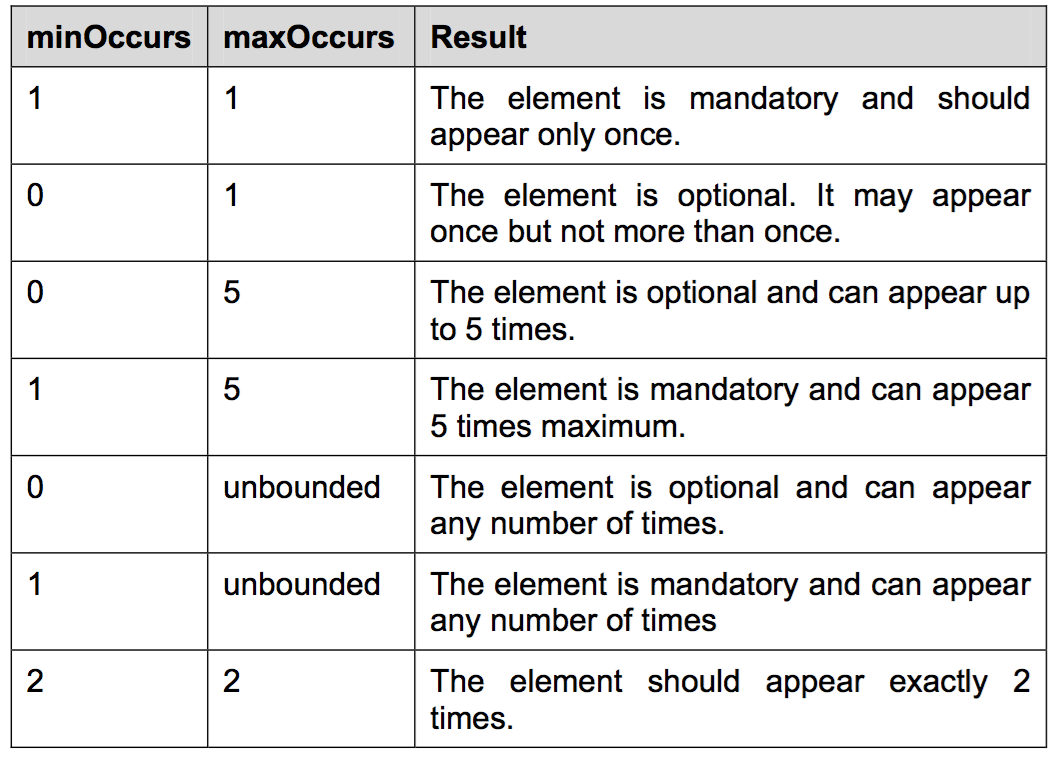
\includegraphics[width=.95\textwidth]{imgs/tabellaMinMaxOccurs.png}
	\end{center}

\end{frame}


%% Element Groups
% provide reusability to a certain extent as they can be inserted into other complex types within the same schema. The schema is easier to modify and maintain.
%% esemipio:
%<xsd:schema xmlns:xsd="http://www.w3.org/2001/XMLSchema">
%   <xsd:group name="ContactInfo">
%     <xsd:sequence>
%       <xsd:element name="email"/>
%       <xsd:element name="phone"/>
%     </xsd:sequence>
%   </xsd:group>
%   <xsd:element name="author">
%     <xsd:complexType>
%       <xsd:sequence>
%         <xsd:group ref="ContactInfo"/>
%       </xsd:sequence>
%    </xsd:complexType>
%   </xsd:element>
% </xsd:schema>
% Una possibile istanza di documento XML validata dallo schema di cui sopra:
% <author>
%       <email>name@institution.it</email>
%       <phone>0039123456789</phone>
% </author>



% Complex type derivation

\begin{frame}
	\frametitle{Elementi per la definizione degli schemi xml}
	\framesubtitle{principi XSD}
	\addtocounter{nframe}{1}

	\begin{block}{Content Model: Deriving}
		Nuovi tipi complessi possono essere derivati da tipi complessi con modello del contentuo Simple Content.
		\textit{Non è possibile derivare Compex Content da Simple Content.}
	\end{block}

	\begin{block}{Content Model: Complex Content}
		Un elemento con modello Complex Content può contenere elementi figli, attributi e testo.
	\end{block}
\end{frame}

% Complex Type derivation
\begin{frame}
	\frametitle{Elementi per la definizione degli schemi xml}
	\framesubtitle{principi XSD}
	\addtocounter{nframe}{1}

	\begin{block}{Content Model: Complex Content}
		\textbf{Nuovi complex types possono essere derivati da complex type già definiti \textit{by restriction} oppure \textit{by extension}}
	\end{block}
\end{frame}

\begin{frame}
	\frametitle{Elementi per la definizione degli schemi xml}
	\framesubtitle{principi XSD}
	\addtocounter{nframe}{1}

	\begin{block}{Complex Type derivation: da simple type}
		E' possibile derivare complex type da un tipo base simple type, ma solo se l'elemento è simple content.
		\\Se l'attributo \textit{final} è impostato sul valore \textbf{extension}, il tipo base (simple type) non può essere esteso.

	\end{block}

\end{frame}

\begin{frame}
	\frametitle{Elementi per la definizione degli schemi xml}
	\framesubtitle{principi XSD}
	\addtocounter{nframe}{1}

	\begin{block}{Complex Type derivation: da simple type - esempio}
		\texttt{
			<xsd:complexType name=``divTypeEx''>
			\emph{<xsd:simpleContent>}
			\emph{<xsd:extension base=``divType''>}
			\emph{<xsd:attribute name=``type'' use=``required''/>}
			</xsd:extension>
			</xsd:simpleContent>
			</xsd:complexType>
		}
	\end{block}
\end{frame}

\begin{frame}
	\frametitle{Elementi per la definizione degli schemi xml}
	\framesubtitle{principi XSD}
	\addtocounter{nframe}{1}

	\begin{block}{Complex Type derivation: Diversi casi}
		\begin{itemize}
			\item derivare un nuovo tipo by restriction oppure by extension da un complex type simple content model
			\item derivare by restriction da un complex type con simple content
			\item aggiungere restrizioni al content/text di un elemento
			\item aggiungere restrizioni ad un attributo
			\item eleminare uno o più attributi ad un tipo di elemento
		\end{itemize}
	\end{block}
	\textit{Le politiche di derivazione cambiano a seconda del modello di contenuto del tipo considerato}

\end{frame}

%% Esempio:
\begin{frame}
	\frametitle{Elementi per la definizione degli schemi xml}
	\framesubtitle{principi XSD}
	\addtocounter{nframe}{1}

	\begin{block}{Complex Type derivation: esempio}
		\texttt{
		<xsd:complexType name=``RestrictedPhoneType''>
		\emph{<xsd:simpleContent>}
		\emph{<xsd:restriction base=``PhoneType''>}
		<xsd:pattern value="[0-9]{3}-[0-9]{3}-[0-9]{4}"/>
		\emph{<xsd:attribute name=``Type''>}
		\emph{<xsd:simpleType>}
		<xsd:restriction base=``xsd:string''>
		<xsd:enumeration value="Home"/>
		<xsd:enumeration value="Work"/>
		</xsd:restriction>
		</xsd:simpleType>
		</xsd:attribute>
		\emph{<xsd:attribute name="CallOnWeekend" type="xsd:boolean" use="prohibited"/> }
		</xsd:restriction>
		</xsd:simpleContent>
		</xsd:complexType>
		}
	\end{block}
\end{frame}


\begin{frame}
	\frametitle{Elementi per la definizione degli schemi xml}
	\framesubtitle{principi XSD}
	\addtocounter{nframe}{1}

	\begin{block}{Complex Type derivation}
		Si noti l'attributo \textbf{use} con valore \textit{prohibited}.
		\\ Se si vuole eliminare un attributo è necessario ridefinirlo nel tipo derivato e impostare l'attributo \textit{use} al valore \textit{prohibited}.
	\end{block}

	\begin{block}{Complex Type derivation}
		Se un attributo è obbligatorio \textit{required} nel tipo base, non è possibile cambiarlo in \textit{optional} nel tipo derivato (non è possibile avere un tipo derivato meno restrittivo del tipo base).
	\end{block}
\end{frame}

\begin{frame}
	\frametitle{Elementi per la definizione degli schemi xml}
	\framesubtitle{principi XSD}
	\addtocounter{nframe}{1}

	\begin{block}{Complex Type derivation}
		\textbf{ Quando si deriva by extension da un tipo complesso con simple content, il tipo risultante sarà sempre un simple content.}
	\end{block}

	\textit{L'unca cosa che è possibile fare è aggiungere attributi}

\end{frame}


\begin{frame}
	\frametitle{Elementi per la definizione degli schemi xml}
	\framesubtitle{principi XSD}
	\addtocounter{nframe}{1}

	\begin{block}{Complex Type derivation: simple content esempio}
		\texttt{
			<xsd:complexType name=``ExtendedPhoneType''>
			\emph{<xsd:simpleContent>}
			\emph{<xsd:extension base=``PhoneType''>}
				<xsd:attribute name="CallOnHolidays" type="xsd:string"/>
			</xsd:extension>
			</xsd:simpleContent>
			</xsd:complexType>
		}
	\end{block}


\end{frame}

%% esempio:
% <xsd:complexType name="ExtendedPhoneType">
%   <xsd:simpleContent>
%     <xsd:extension base="PhoneType">
%       <xsd:attribute name="CallOnHolidays" type="xsd:string"/>
%     </xsd:extension>
%   </xsd:simpleContent>
% </xsd:complexType>


\begin{frame}
	\frametitle{Elementi per la definizione degli schemi xml}
	\framesubtitle{principi XSD}
	\addtocounter{nframe}{1}

	\begin{block}{Complex Type derivation}
		Un tipo complesso \textit{element-only content} può essere esteso (extended) o limitato (restricted) per generare un nuovo tipo.
	\end{block}

	\begin{block}{Complex Type derivation}
		Derivare \textit{by restriction} da un tipo \textit{element-only content} vuol dire eliminare elementi o attributi.
		\\\textbf{Attenzione: gli elementi del tipo di base non vengono passati al tipo derivato (a differenza degli attributi)}
	\end{block}
\end{frame}


\begin{frame}
	\frametitle{Elementi per la definizione degli schemi xml}
	\framesubtitle{principi XSD}
	\addtocounter{nframe}{1}

		%\textbf{Tutti gli elementi obbligatori nel tipo di base devono essere presenti anche nel tipo derivato}
	
	\begin{block}{Complex Type derivation}
		\begin{itemize}
			\item Se gli elementi nel tipo di base sono dichiarati all'interno di una \textit{sequence}, il tipo derivato non può cambiare tale dichiarazione in \textit{all} oppure \textit{choice}.
			\item Se il tipo di base ha specificato gli elementi con una dichiarazione \textit{all}, il tipo derivato può cambiare la dichiarazione con \textit{sequence}. 
			\item Se il tipo di base ha specificato gli elementi con la dichiarazione \textit{choice}, il tipo derivato deve avere ugualmente la dichiarazione \textit{choice}.
		\end{itemize}
	\end{block}
\end{frame}

\begin{frame}
	\frametitle{Elementi per la definizione degli schemi xml}
	\framesubtitle{principi XSD}
	\addtocounter{nframe}{1}

	
	\begin{block}{Complex Type derivation}
		\begin{itemize}
			\item Se si vuole rimuovere un attributo bisogna dichiararlo nuovamente e specificarne l'uso \textit{prohibited}.
			\item Un tipo derivato non può eliminare un attributo dichiarato obbligatorio nel tipo di base.
			\item Bisogna ridefinire un attributo nel tipo derivato, solo se si vuole limitare il suo spazio di valori (\textit{gli attributi vengono ereditati dal tipo derivato}).
		\end{itemize}
	\end{block}
\end{frame}


% Esempio:

\begin{frame}
	\frametitle{Elementi per la definizione degli schemi xml}
	\framesubtitle{principi XSD}
	\addtocounter{nframe}{1}

	\begin{block}{Complex Type derivation: esempio}
		%   <!-- Contact Element -->
		\texttt{\emph{<xsd:element name="Contact" type="RestrictedContactType"/>}}
		\\\texttt{%<!-- Contact Type -->
			<xsd:complexType name=``ContactType''>
			<xsd:sequence>
			<xsd:element name="Phone" minOccurs="0"/>
			<xsd:element name="Email" minOccurs="0"/>
			</xsd:sequence>
			<xsd:attribute name="Name" />
			<xsd:attribute name="Title"/>
			</xsd:complexType>}
	\end{block}
\end{frame}

\begin{frame}
	\frametitle{Elementi per la definizione degli schemi xml}
	\framesubtitle{principi XSD}
	\addtocounter{nframe}{1}

	\begin{block}{Complex Type derivation: esempio}
		%<!-- Restricted Contact Type -->
		\texttt{<xsd:complexType name=``RestrictedContactType''>
		\emph{<xsd:complexContent>}
		\emph{<xsd:restriction base=``ContactType''>}
		<xsd:sequence>
		<xsd:element name=``Phone''>
		<xsd:simpleType>
		<xsd:restriction base=``xsd:string''>
		<xsd:pattern value="[0-9]{3}-[0-9]{3}-[0-9]{4}"/>
		</xsd:restriction>
		</xsd:simpleType>
		</xsd:element>
		</xsd:sequence>
		\emph{<xsd:attribute name="Title" use="prohibited"/>}
		\emph{<xsd:attribute name=``Name'' type=``xsd:string''>}
		</xsd:attribute>
		</xsd:restriction>
		</xsd:complexContent>
		</xsd:complexType>}
	\end{block}
\end{frame}


\begin{frame}
	\frametitle{Elementi per la definizione degli schemi xml}
	\framesubtitle{principi XSD}
	\addtocounter{nframe}{1}

	\begin{block}{Complex Type derivation}
		E' possibile derivare un \textit{empty content} da un\textit{ element-only content}. 
		\\Ciò viene fatto mantenendo la \textit{dichiarazione di restrizione vuota}. 
		\\Questo \textbf{non vale per gli attributi}, che si ereditano tutti.
	\end{block}

	\begin{block}{Complex Type derivation}
		\textbf{Gli elementi del tipo dell'elemento base devono essere opzionali}
	\end{block}
\end{frame}


\begin{frame}
	\frametitle{Elementi per la definizione degli schemi xml}
	\framesubtitle{principi XSD}
	\addtocounter{nframe}{1}

	\begin{block}{Complex Type extension}
		\textit{I tipi \textbf{complex type} vengono estesi per aggiungere elementi e attributi}
	\end{block}

	\begin{block}{Complex Type extension}
		\textbf{Quando si deriva per estensione, sia tutti gli elementi, sia tutti gli attributi si ereditano dal tipo base al tipo derivato}.
	\end{block}
\end{frame}


% <xsd:schema xmlns:xsd="http://www.w3.org/2001/XMLSchema">
%   <!-- Contact Element -->
%   <xsd:element name="Contact" type="ExtendedContactType"/>
%   
%   <!-- Extended Contact Type -->
%   <xsd:complexType name="ExtendedContactType">
%     <xsd:complexContent>
%       <xsd:extension base="ContactType">
%         <xsd:sequence>
%           <xsd:element name="Fax"/>
%         </xsd:sequence>
%         <xsd:attribute name="Department"/>
%       </xsd:extension>
%     </xsd:complexContent>
%   </xsd:complexType>
%  
%    <!-- Contact Type -->
%   <xsd:complexType name="ContactType">
%     <xsd:sequence>
%       <xsd:element name="Phone"/>
%       <xsd:element name="Email" minOccurs="0"/>
%     </xsd:sequence>
%     <xsd:attribute name="Name" use="required"/>
%     <xsd:attribute name="Title"/>
%   </xsd:complexType>
% </xsd:schema>
%
%% Una possibile istanza XML:
% <Contact Name="Jacob" Title="Manager" Department="IT">
%   <Phone>999-888-7777</Phone>
%   <Email>jacob@jacob.com</Email>
%   <Fax>888-999-3333</Fax>
% </Contact>

\begin{frame}
	\frametitle{Elementi per la definizione degli schemi xml}
	\framesubtitle{principi XSD}
	\addtocounter{nframe}{1}

	\begin{block}{Complex Type derivation: esempio}
		%   <!-- Contact Element -->
		\texttt{\emph{<xsd:element name="Contact" type="ExtendedContactType"/>}}
		\texttt{%<!-- Contact Type -->
			<xsd:complexType name=``ContactType''>
			<xsd:sequence>
			<xsd:element name=``Phone''/>
			<xsd:element name=``Email'' minOccurs=``0''/>
			</xsd:sequence>
			<xsd:attribute name=``Name'' use=``required''/>
			<xsd:attribute name=``Title''/>
			</xsd:complexType>
			</xsd:schema>
		}
	\end{block}
\end{frame}


\begin{frame}
	\frametitle{Elementi per la definizione degli schemi xml}
	\framesubtitle{principi XSD}
	\addtocounter{nframe}{1}

	\begin{block}{Complex Type derivation: esempio}
		%<!-- Extended Contact Type -->
		\texttt{
			<xsd:complexType name=``ExtendedContactType''>
			\emph{<xsd:complexContent>}
			\emph{<xsd:extension base=``ContactType''>}
			<xsd:sequence>
			\emph{<xsd:element name=``Fax''/>}
			</xsd:sequence>
			\emph{<xsd:attribute name=``Department''/>}
			</xsd:extension>
			</xsd:complexContent>
			</xsd:complexType>
		}
	\end{block}
\end{frame}

\begin{frame}
	\frametitle{Elementi per la definizione degli schemi xml}
	\framesubtitle{principi XSD}
	\addtocounter{nframe}{1}

	\begin{block}{Complex Type: deriving }
		Si può derivare un \textit{mixed content} sia by restriction sia by extension.
		Derivare un tipo complesso \textit{mixed content} è simile a derivare un tipo complesso \textit{element-only}.
	\end{block}

	\begin{block}{Complex Type: deriving}
		 deriving by restriction un mixed content type: \textit{a mixed type}, \textit{element-only} oppure \textit{empty content}. 
	\end{block}
	\textit{Gli elementi dichiarati nel tipo base non si ereditano, gli attributi si ereditano}
\end{frame}


% esempio:
\begin{frame}
	\frametitle{Elementi per la definizione degli schemi xml}
	\framesubtitle{principi XSD}
	\addtocounter{nframe}{1}

	\begin{block}{Complex Type derivation: esempio}
		%<!-- Extended Contact Type -->
		\texttt{
			\emph{<xsd:complexType name="RestrictedNoteType" mixed=``true''>}
			\emph{<xsd:complexContent>}
			\emph{<xsd:restriction base=``NoteType''>}
			<xsd:sequence>
			<xsd:element name="name"/>
			</xsd:sequence>
			</xsd:restriction>
			</xsd:complexContent>
			</xsd:complexType>
		}
	\end{block}
	\textit{Rimuovendo l'attributo ``mixed'' dalla dichiarazione del tipo complesso si ottiene un element-only complex type da un tipo mixed content}
\end{frame}

\begin{frame}
	\frametitle{Elementi per la definizione degli schemi xml}
	\framesubtitle{principi XSD}
	\addtocounter{nframe}{1}
	\begin{block}{Complex Type: deriving - Mixed Content}
		Quando si deriva by restriction un mixed type, si può creare un \textit{empty content type} se tutti gli elementi del tipo base sono optionali. 
	\end{block}
	\begin{block}{Complex Type: deriving - Mixed Content}
		Per eliminare gli attributi c'è bisogno di dichiararli nel tipo derivato e di proibirne l'uso (\textit{prohibited attribute}).
	\end{block}
\end{frame}

% esempio
\begin{frame}
	\frametitle{Elementi per la definizione degli schemi xml}
	\framesubtitle{principi XSD}
	\addtocounter{nframe}{1}

	\begin{block}{Complex Type derivation: esempio}
		\texttt{
			\emph{<xsd:complexType name=``SimpleNoteType''>}
			\emph{<xsd:simpleContent>}
			<xsd:restriction base=``NoteType''>
			<xsd:simpleType>
			\emph{<xsd:restriction base="xsd:string"/>}
			</xsd:simpleType>
			</xsd:restriction>
			</xsd:simpleContent>
			</xsd:complexType>
		}
	\end{block}
	\textit{Le specifiche XSD permettono di derivare un simple content da un mixed-content type}
\end{frame}

% esempio
\begin{frame}
	\frametitle{Elementi per la definizione degli schemi xml}
	\framesubtitle{principi XSD}
	\addtocounter{nframe}{1}

	\begin{block}{Complex Type derivation: esempio}
		%   <!-- Note Type -->
		\texttt{
			<xsd:complexType name=``NoteType'' mixed=``true''>
			<xsd:sequence>
			<xsd:element name="name"/>
			<xsd:element name="mobile"/>
			</xsd:sequence>
			</xsd:complexType>
		}
	\end{block}
	\textit{Quando si deriva by \textbf{extension}, possiamo solo generare \textbf{mixed content complex type}}
\end{frame}


\begin{frame}
	\frametitle{Elementi per la definizione degli schemi xml}
	\framesubtitle{principi XSD}
	\addtocounter{nframe}{1}

	\begin{block}{Complex Type derivation: esempio}
		\texttt{\emph{<xsd:element name="InvoiceNote" type="ExtendedNoteType"/>}}


		%!-- Extended Note Type -->
		\texttt{
			<xsd:complexType name=``ExtendedNoteType'' mixed=``true''>
			\emph{<xsd:complexContent>}
			\emph{<xsd:extension base=``NoteType''>}
			<xsd:sequence>
			<xsd:element name=``email''/>
			</xsd:sequence>
			</xsd:extension>
			</xsd:complexContent>
			</xsd:complexType>
		}
	\end{block}
\end{frame}

\begin{frame}
	\frametitle{Elementi per la definizione degli schemi xml}
	\framesubtitle{principi XSD}
	\addtocounter{nframe}{1}

	\begin{block}{Complex Type derivation: esempio}
		%   Una possibile istanza XML
		\texttt{
			<InvoiceNote>
			Chiamare <name>Angelo</name> sul numero di cellulare <mobile>0039 321 32321</mobile> or <email>angelo.delgrosso@ilc.cnr.it</email> se l'ordine non va a buon fine.
			</InvoiceNote>
		}
	\end{block}
\end{frame}

\begin{frame}
	\frametitle{Elementi per la definizione degli schemi xml}
	\framesubtitle{principi XSD}
	\addtocounter{nframe}{1}

	\begin{block}{Complex Type extension}
		\textbf{si può derivare un nuovo tipo da un elemento di tipo \textit{empty content} sia by restriction sia by extension}
	\end{block}

	\begin{block}{Complex Type extension}
		Un elemento con \textit{empty content} ha solo attributi, l'unico motivo per derivare da questa tipologia di content model by restriction è quella di eliminare attributi oppure aggiungere restrizioni.
	\end{block}
\end{frame}



%% esempio:
% <xsd:complexType name="RestrictedPhoneType">
%   <xsd:complexContent>
%     <xsd:restriction base="PhoneType">
%       <xsd:attribute name="Work" use="prohibited"/>
%       <xsd:attribute name="Home">
%         <xsd:simpleType>
%           <xsd:restriction base="xsd:string">
%             <xsd:pattern value="[0-9]{3}-[0-9]{3}-[0-9]{4}"/>
%           </xsd:restriction>
%         </xsd:simpleType>
%       </xsd:attribute>
%     </xsd:restriction>
%   </xsd:complexContent>
% </xsd:complexType>


\begin{frame}
	\frametitle{Elementi per la definizione degli schemi xml}
	\framesubtitle{principi XSD}
	\addtocounter{nframe}{1}

	\begin{block}{Complex Type extension}
		\textbf{Quando si deriva by extension è possibile generare empty type, mixed type oppure element only content type.}
	\end{block}

\end{frame}


\begin{frame}
	\frametitle{Elementi per la definizione degli schemi xml}
	\framesubtitle{principi XSD}
	\addtocounter{nframe}{1}

	\begin{block}{Complex Type derivation: esempio}

		\texttt{
			<xsd:complexType name=``ElemOnlyPhoneType''>
			\emph{<xsd:complexContent>}
			\emph{<xsd:extension base=``EmptyPhoneType''>}
			<xsd:sequence>
			\emph{<xsd:element name=``Mobile''/>}
			</xsd:sequence>
			</xsd:extension>
			</xsd:complexContent>
			</xsd:complexType>
		}
	\end{block}
	\textit{Si può derivare un element only content type da un empty content type by extension}
\end{frame}


\begin{frame}
	\frametitle{Elementi per la definizione degli schemi xml}
	\framesubtitle{principi XSD}
	\addtocounter{nframe}{1}

	\begin{block}{Complex Type derivation: esempio}

		\texttt{
			\emph{<xsd:complexType name=``MixedPhoneType'' mixed=``true''>}
			<xsd:complexContent>
			\emph{<xsd:extension base=``EmpyPhoneType''>}
			<xsd:sequence>
			\emph{<xsd:element name="Mobile"/>}
			</xsd:sequence>
			</xsd:extension>
			</xsd:complexContent>
			</xsd:complexType>
		}
	\end{block}
	\textit{Si può derivare un mixed content type da un empty content type by extension}
\end{frame}

\begin{frame}
	\frametitle{Elementi per la definizione degli schemi xml}
	\framesubtitle{principi XSD}
	\addtocounter{nframe}{1}

	\begin{block}{Complex Type derivation: esempio}

		\texttt{
			<Phone Home=``888-888-8888'' Work=``777-777-7777''>
			Se non disponibile contattare il cellulare al numero
			<Mobile>666-666-6666</Mobile>.
			</Phone>
		}
	\end{block}
\end{frame}




\begin{frame}
	\frametitle{Elementi per la definizione degli schemi xml}
	\framesubtitle{principi XSD}
	\addtocounter{nframe}{1}

	\begin{block}{Derivazione: riepilogando}

		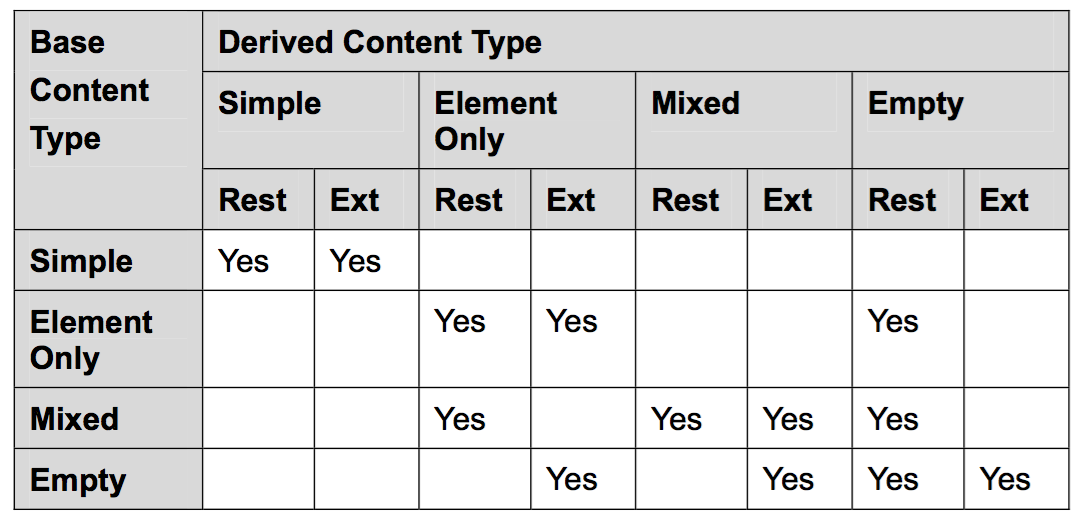
\includegraphics[width=.95\textwidth]{imgs/TabellaContentTypeDerivation.png}

	\end{block}

	\begin{tiny}
		\textit{Nuovi complex types possono essere creati a partire da altri complex types by extension and restriction.}
	\end{tiny}
\end{frame}



\begin{frame}
	\frametitle{Elementi per la definizione degli schemi xml}
	\framesubtitle{principi XSD}
	\addtocounter{nframe}{1}

	\begin{block}{Complex Type derivation: final attribute}
		\textbf{La derivazione di un tipo complesso può essere controllata impiegando l'attributo final nella dichiarazione del tipo}
	\end{block}

\end{frame}

\begin{frame}
	\frametitle{Elementi per la definizione degli schemi xml}
	\framesubtitle{principi XSD}
	\addtocounter{nframe}{1}

	\begin{block}{Complex Type derivation: final attribute}
		\textit{L'attributo final può assumere i seguenti valori:}
		\begin{itemize}
			\item \textbf{restriction}: limita la derivazione by restriction
			\item \textbf{extension}: limita la derivazione by extension
			\item \textbf{\#all}: limita la derivazione by restriction e by extension
		\end{itemize}

	\end{block}

\end{frame}

% esempio: how to control the derivation of a given complex type: 
\begin{frame}
	\frametitle{Elementi per la definizione degli schemi xml}
	\framesubtitle{principi XSD}
	\addtocounter{nframe}{1}

	\begin{block}{Complex Type derivation: esempio}

		\texttt{
			\emph{<xsd:complexType name=``ContactType'' final=``extension restriction''>}
			<xsd:sequence>
			<xsd:element name="Phone" minOccurs="0"/>
			</xsd:sequence>
			<xsd:attribute name="Name" />
			</xsd:complexType>
		}
	\end{block}
\end{frame}

\begin{frame}
	\frametitle{Elementi per la definizione degli schemi xml}
	\framesubtitle{principi XSD}
	\addtocounter{nframe}{1}

	\begin{block}{Complex Type derivation: esempio - derivazione non consentita}

		\texttt{
			<xsd:complexType name=``ExtendedContactType''>
			\emph{<xsd:complexContent>}
			\emph{<xsd:extension base="ContactType"/>}
			</xsd:complexContent>
			</xsd:complexType>
		}
	\end{block}
\end{frame}

